\documentclass[a4paper,openany]{uantwerpenassignment}

\usepackage[dutch]{babel}
\usepackage{titlesec}
\usepackage{tikz}

\facultyacronym{TI}

\title{\sffamily Chess AI-Agent}
\subtitle{\sffamily5-Artificiële Intelligentie}
\author{\sffamily Mathias Maes, Tijs Van Alphen \\en Willem Van der Elst}

\programme{BA}{IW}{EI}

\academicyear{2020-2021}

\publisher{}

\titleformat{\chapter}{\sffamily\huge\bfseries}{\thechapter.}{10pt}{\sffamily\huge\bfseries}
\titleformat{\section}{\sffamily\LARGE\bfseries}{\thesection.}{10pt}{\sffamily\LARGE\bfseries}
\titleformat{\subsection}{\sffamily\Large\bfseries}{\thesubsection.}{10pt}{\sffamily\Large\bfseries}
\titleformat{\subsubsection}{}{}{10pt}{\sffamily\large\bfseries}


\begin{document}

\sffamily
\maketitle

\tableofcontents

\chapter{Keuze}

Om onze keuze te maken hadden we een lijst opgesteld met positieve en negatieve punten opgesteld.

[VOEG + en - punten toe]

Uit deze lijst hadden we 2 keuzes die voor ons er ver bovenuit staken Q-Learning en Minimax.

Uiteindelijk ging de keuze naar beide agents. We hadden namelijk een thesis\cite{rl} gevonden die een minimax agent gebruikte als feature voor een generalized Q-Learner.

\chapter{Q-Learning Agent}

\section{Generalization}

De eerste agent die we moesten maken was de Q-Learner deze is generalized omdat zoals bij de minpunten stonden van general search algoritmes, is het bijna onmogelijk om elke staat te bezoeken. Daarom dat we niet gewoon Q-Learning gaan doen maar generalized Q-Learning.

\section{Features}

We hebben een hoop features gedefinieerd deze zijn voornamelijk gebaseerd op de paper\cite{rl} die we gevonden hebben. De bedoeling van deze features is om een state zo goed mogelijk te definiëren. Je kan hieronder een beschrijving vinden van elks van onze 55 features.

We berekenen onze features als volt:

$$
Q(s,a) = \sum_{i} w_{i} \cdot \sigma \left( f_i(s, a)\right)
$$

De $\sigma(x)$ die we in de berekening zien wordt als volgt gedefinieerd:

$$
\sigma(x) = \frac{2}{1 + e^{-x}} - 1
$$


Dit is een aangepaste versie van de bekende sigmoid\cite{WSF} functie. Onze versie zorgt in tegenstelling tot de originele er voor dat waardes in het interval $\left]-1,1\right[$ vallen.\\
Hier zie je de grafiek van de functie:

\begin{figure}[h]
    \centering
    \begin{tikzpicture}[scale=2]
        \draw[->] (-2, 0) -- (2, 0) node[right] {$x$};
        \draw[->] (0, -1.2) -- (0, 1.2) node[above] {$y$};

        \draw[dashed] (-2, 0.5) -- (2, 0.5);
        \node (A) at (-2, 0.6) {\tiny $1$};

        \draw[dashed] (-2, -0.5) -- (2, -0.5);
        \node (B) at (-2, -0.6) {\tiny $-1$};

        \draw[scale=0.5, domain=-3.9:3.9, smooth, variable=\x, blue] plot ({\x}, { 2/(1 + exp(-\x)) - 1 });
        \node[blue] (C) at (0.4, 0.32) {$\sigma$};
    \end{tikzpicture}
    \caption{$\sigma(x)$} \label{fig:sigmoid}
\end{figure}


\section{Reward}

\chapter{Alpha-Beta Pruning}

\section{Utility}

Evaluation\cite{chessprogramming}

\chapter{Optimalisaties}

We hebben een hoop optimalisaties moeten toevoegen aan onze Q-Learner om hem zo rap mogelijk te laten denken.

\section{Multi-Threading}

We hebben multi-threading toegevoegd aan onze q-learner zo berekent hij de q-waarde van elke actie in een aparte thread. We hebben bewust niet gekozen om elke feature apart omdat dit onze timing issues verergerde in plaat van verbeterde.

Hier zie je de resultaten van het processor gebruik:

\begin{figure}[h]
    \centering
    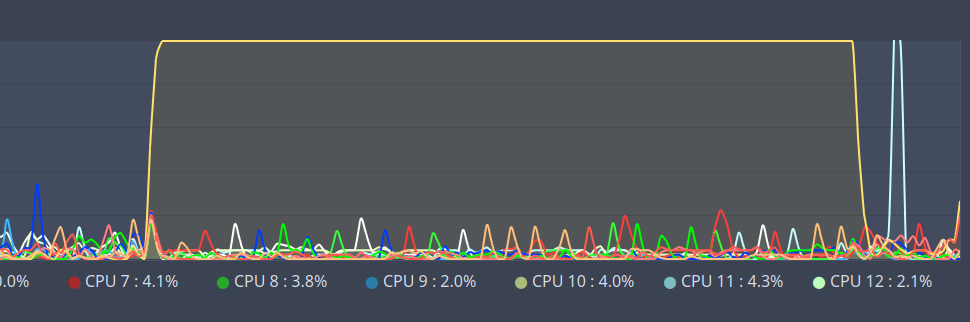
\includegraphics[width=300pt]{images/singlethreaded.png}
    \caption{Single Threaded Q-Learner CPU usage}
    \label{fig:singlethreaded}
\end{figure}

\begin{figure}[h]
    \centering
    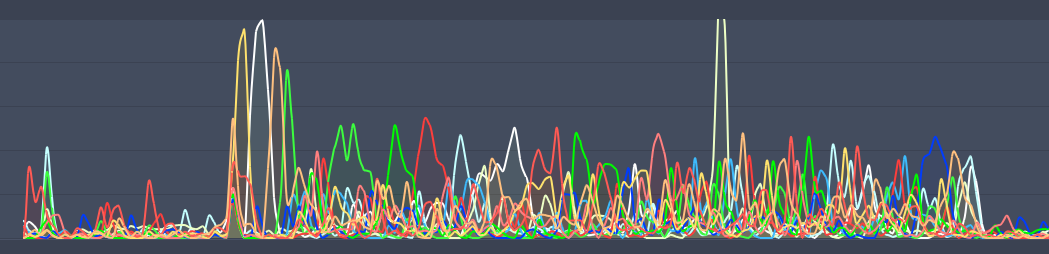
\includegraphics[width=350pt]{images/multithreaded.png}
    \caption{Multi Threaded Q-Learner CPU usage}
    \label{fig:multithreaded}
\end{figure}


% python3 train -o stockfish --skill 0 --depth 10 -tt 5 -dt 0 -e 0.3 -d 0.6 -l 0.01 -q -i -1
% python3 train -o ab --skill 0 --depth 10 -tt 5 -dt 0 -e 0.2 -d 0.4 -l 0.01 -q -i -1

\bibliography{sources}
\bibliographystyle{ieeetr}

\end{document}
